\documentclass[letterpaper,11pt]{article}

\usepackage[paper = letterpaper,
            left = 1in, right= 1in,
            top = 1in, bottom= 1in,
            centering]{geometry}

\usepackage{lmodern}
% Use LaTeX modern fonts, little nicer than the default computer modern.
\usepackage{textcomp}
% Textcomp takes some characters from the T1 encoding.
\usepackage{microtype}
% Gives punctuation at the end of the lines a smoother appearance by character protrusion.
\usepackage{amsmath}
 % Used to attach files (MATLAB scripts)
\usepackage{listings}
\usepackage{moreverb}

% Allows inclusion of bitmap graphics (jpg, png)
\usepackage{pslatex}
\usepackage{graphicx}
% \graphicspath{{../figures/}}

% for drawing circuit diagrams
% \usepackage[americanvoltages]{circuitikz}
% \usepackage{tikz}

\usepackage{hyperref}

% use fancy Header/Footer
\usepackage{fancyhdr}
\pagestyle{fancy}
\usepackage{lastpage}

% Set Header and Footer
\lhead{NEPR 208}
\chead{}
\rhead{Learning and memory}
\lfoot{}
\cfoot{\thepage\ of \pageref{LastPage}}
\rfoot{}
\renewcommand{\headrulewidth}{0.2pt}

% letters in enumerate
\renewcommand{\theenumi}{\Alph{enumi}}

% Horizontal line
\newcommand{\HRule}{\rule{\linewidth}{0.5mm}}

% -- Figure, Float, Table, and List Formatting
\usepackage{array} % tables
\usepackage{float} % place tables in exact positions
% Redefine some parameters of floats
\usepackage{booktabs} % improves the look of tables

% Double Space report
\usepackage{setspace}
\onehalfspacing

% Title Page
\begin{document}

\begin{center}
\thispagestyle{empty}

% Upper part of the page
\textsc{\Large Problem Set 3}\\[0.5cm]

% Title
\HRule \\[0.6cm]
{ \huge \bfseries Learning and Memory}\\[0.2cm]

\HRule \\[2.5cm]

\end{center}
% \tableofcontents

% Report
\section{Hopfield model}
\subsection*{Introduction}
The goal of this problem set is to explore the behavior of the Hopfield model.
Specifically, we are interested in addressing several questions regarding the time it takes to recall a memory and the sizes of basins of attraction in the Hopfield model. 
Make sure to download the Matlab example code \texttt{ExploreHopfield.m} from the course website.
You will modify the code to answer the questions below.

One note about the implementation--you do not have to scan parameters (like number of patterns $P$, and basin of attraction size $K$) at a level of resolution of every $P$ and $K$, as this would take too long.  Feel free to scan them at lower resolution--and also you don't have to scan them over the entire range--only over a range in which interesting quantities like recall probability, overlap, and recall time vary in interesting ways.
Basically, imagine that you are doing research on the Hopfield model, and you have several hypotheses that as the number of stored patterns increase, basins of attraction get smaller and recall probability goes down, and recall time (conditional on successful recall) goes up.
Lets say you want to present numerical evidence for these conjectures in the form some figures for a paper.
Then part of your job would be not only figuring out what to plot (which is outlined in the different parts of the problem) but also over what ranges and what resolution of parameters to plot at (for which we gave initial suggestions that are most likely suboptimal).
So feel free to make your own decisions about what exactly to plot.

\subsection{Basins of Attraction}
First, we will investigate the basins of attraction. Recall that a \textit{basin of attraction} in the Hopfield model is set of neural activity patterns, that when set as the initial condition, all converge to the same attractor state (Figure \ref{fig:energy}). We would like to understand properties of the basins of attraction, because they directly correspond to how corrupt a recoverable memory can be. Here, we will explore how big the basins of attraction are as a function of the number of patterns in the network ($P$) and the amount of corruption ($K$).

In class, we talked through an example with only $N$ = 3 neurons, where it was very easy to
see how ``corrupted'' a pattern was by counting the number of mismatched places. Here, when we
simulate larger networks, we'll need an automatic way to quantify how close two activity patterns u
and v are. For this, we'll use overlap, defined as $\frac{1}{N} \sum_{i=1}^N u_i v_i = \frac{1}{N} (u_1 v_1 + u_2 v_2 + \cdots + u_N v_N)$. This is always a number between -1 and 1, where 1 indicates perfect overlap - ie. all places match. (This measure is closely related to the pearson correlation coefficient between the two patterns.)

\begin{figure}[h!]
  \begin{center}
    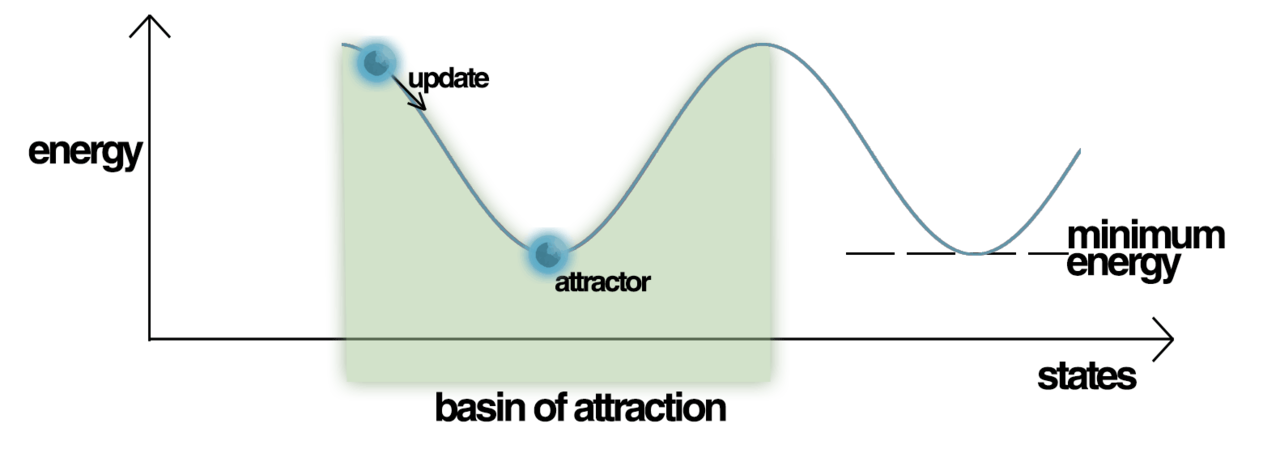
\includegraphics[width=0.6\textwidth]{energy.png}
    \caption{Energy Landscape of a Hopfield Network. The memories in the network are attractor states (local minima) of the energy landscape. Given an initial condition (e.g. a partial memory) in a particular basin of attraction, the dynamics of the network are such that the network settles at the attractor. \textit{(Image from \href{http://www.wikiwand.com/en/Hopfield\_network}{Wikipedia})}}
    \label{fig:energy}
  \end{center}
\end{figure}

\begin{enumerate}
  \item The code (see lines 15-17) fixes $P$ random patterns stored in a Hopfield network of size $N=1000$ by defining the network connectivity ($J$) as the outer product of the patterns. If you run the code, it will build the Hopfield network, initialize the network at either a random location (if \texttt{InitCondType} is 1) or at a location that is $K$ bit flips away from one of the original patterns (if \texttt{InitCondType} is 2), and finally run the dynamics of the network. There is code at the bottom that visualizes the overlap of the current network state with each of the learned patterns. Successful recall occurs when, after running the dynamics, when the network is attracted to one of the input patterns (one of the overlap bars should shoot up close to 1, as in Figure \ref{fig:recall}). With \texttt{InitCondType} set to 2, verify that the network successfully recalls a stored pattern (we will define successful recall if the final maximum overlap is at least 0.9). If you increase the number of patterns, $P$, to 200, does the network recall the pattern?
  \item For $P$ ranging from 20 to 600, start the network from an initial condition consisting of $K$ bit flips away from a randomly chosen stored pattern (\texttt{InitCondType} = 2) for $K$ ranging from 1 to 500 (you don't need to test every value in this range), and check to see if the network goes back to the stored pattern--i.e. if the fixed point that the network arrives at has overlap $> 0.9$ with the stored pattern (the variable \texttt{successful\_recall} computes this). You will have to write your own \texttt{for} loops to accomplish this. You do not need to test every value of $P$ and $K$ in the range--for example, in Matlab, you can use \texttt{for P=20:5:600} to scan $P$ from 20 to 600 in steps of 5, for example. For $K=1$, around what value of $P/N$ does the system transition from successful to failed recall? As $K$ gets bigger, does this critical $P/N$ value increase, decrease, or stay the same?
  \item For each $K$ and $P$, repeat this procedure multiple times (say for $\geq 100$ trials) to estimate the probability that a network will be able to recall a stored pattern from a corrupted version. Plot this probability as a heat map (using the \texttt{imagesc} or \texttt{pcolor} commands) as a function of $K/N$ and $P/N$. This will give you an indication of how the size of basins of attraction shrinks as the number of stored patterns increases. Also, by plotting this in terms of the ratios, you obtain a plot that would remain roughly invariant if you changed $N$.
  \item Bonus: perform the same analysis for larger $N$ (say, $N$ = 2000). How does the capacity
change for any given fixed K? More generally, how would you expect the memory capacity
of the hopfield network to scale with the number of neurons?.
  % \item Instead of plotting the probability that the overlap with the chosen stored pattern is $> 0.9$, plot also the mean overlap with the chosen stored pattern across trials as a heat map as a function of $K/N$ and $P/N$. This provides a view of the location of nearby valleys in the energy landscape (valleys near the one containing the uncorrupted chosen pattern).
\end{enumerate}

\begin{figure}[h!]
  \begin{center}
    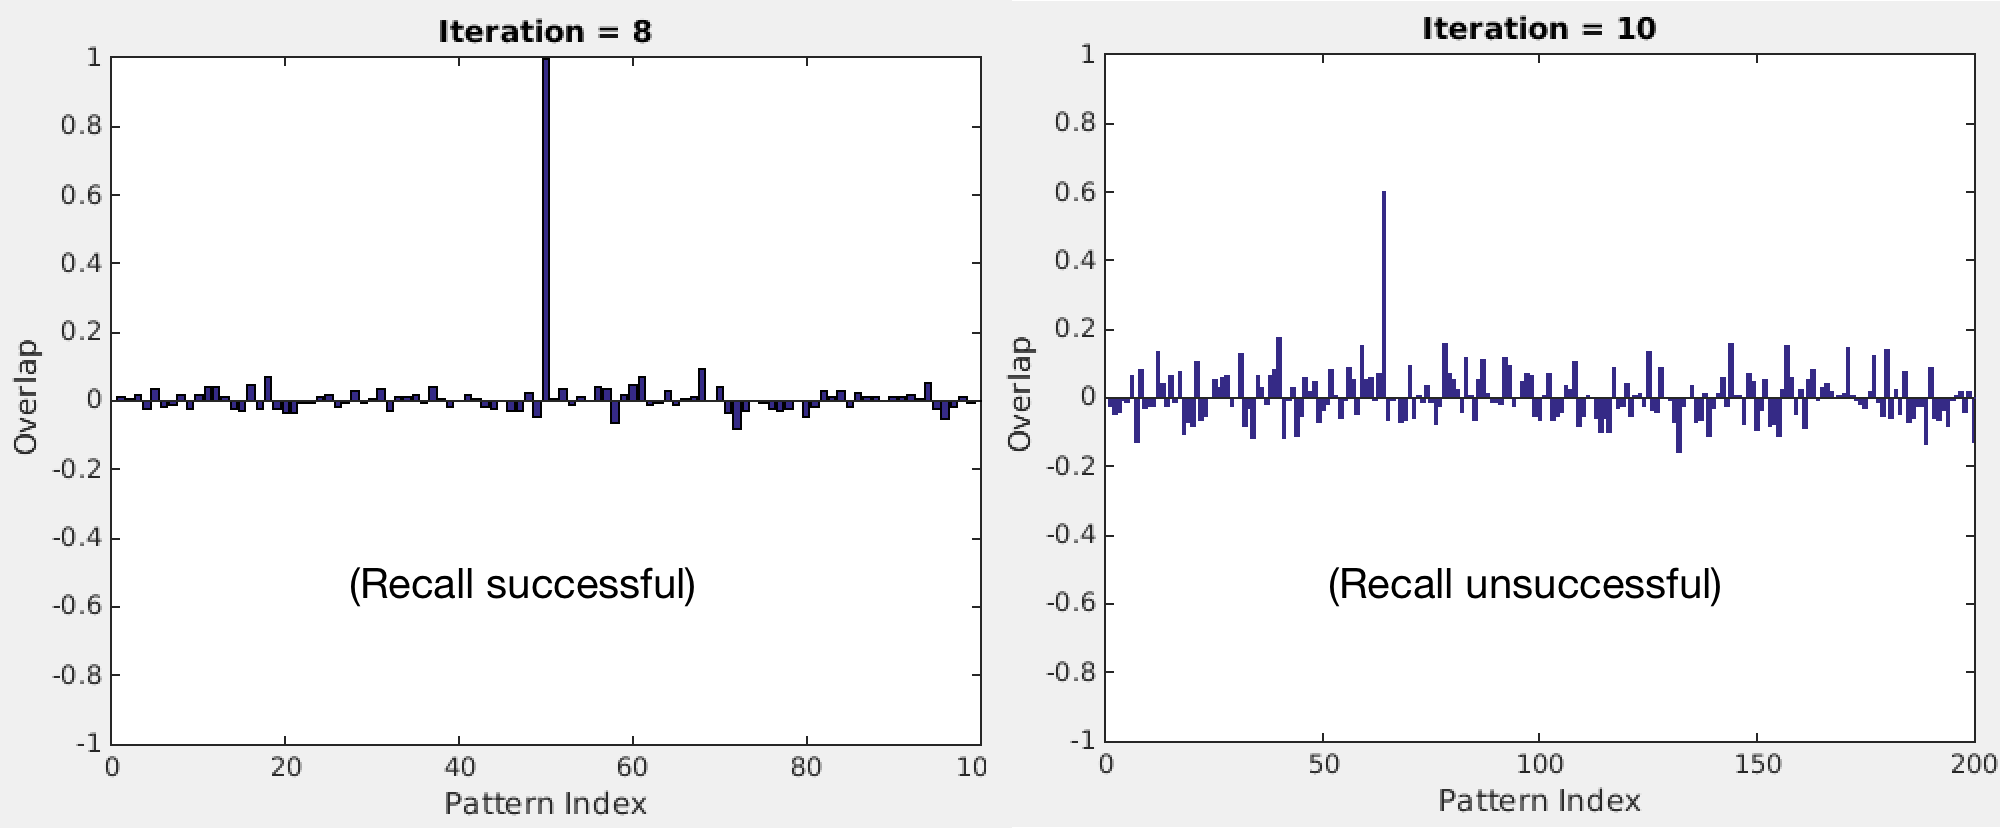
\includegraphics[width=0.7\textwidth]{recall.png}
    \caption{Successful (left) and unsuccessful (right) memory recall in a Hopfield model.}
    \label{fig:recall}
  \end{center}
\end{figure}

\subsection{Recall probability and recall time (extra credit)}
Local minima of the energy function are memories of the Hopfield network.
Although our learned (desired) patterns are local minima, there are also spurious local minima.
Next, we will look at the probability that we recall one of the original $P$ patterns given a random initial condition (as opposed to a spurious local minima).
This is the \textit{recall probability}.
We will also look at the \textit{recall time}, the number of update steps required to reach one of the existing patterns.
Note that this problem is extra credit.

\begin{enumerate}
  \item Again, we will start with $P$ random patterns stored in a Hopfield network of size $N=1000$. For $P$ ranging from 20 to 600, run the network multiple times (say 100 times) from a completely random initial condition (\texttt{InitCondType} = 1). Record the fraction of times that the network achieves a recall state (just like before, if the final state has a large overlap ($> 0.9$ in absolute value)) with one of the $P$ patterns. Plot this fraction as a function of $P/N$.
  \item Also, plot the mean and standard deviation (across trials in which a recall state was found) of the \textit{time} (number of iterations of the dynamics) it takes to find a recall state, as a function of $P$. This plot will terminate as some early value of $P$ because at larger values, the network will never be able to find a recall state from a random initial condition.
  \item What is the relationship between the recall time and recall probability?
\end{enumerate}

\bibliographystyle{plain}
\bibliography{../../references.bib}

\end{document}
